%%%%%%%%%%%%%%%%%%%%%%%%%%%%%%%%%%%%%%%%%%%%%%%%%%%%%%%%%%%%
\documentclass[xcolor=x11names,compress]{beamer}

\definecolor{CoolBlack}{rgb}{0.0, 0.18, 0.39}
\definecolor{byellow}{rgb}{0.55037, 0.38821, 0.06142}
%% General document %%%%%%%%%%%%%%%%%%%%%%%%%%%%%%%%%%
\usepackage{graphicx}
\usepackage{tikz}
\usepackage{Tabbing}
\usetikzlibrary{decorations.fractals}
%%%%%%%%%%%%%%%%%%%%%%%%%%%%%%%%%%%%%%%%%%%%%%%%%%%%%%

%% Beamer Layout %%%%%%%%%%%%%%%%%%%%%%%%%%%%%%%%%%
\useoutertheme[subsection=false,shadow]{miniframes}
\useinnertheme{default}
\usefonttheme{serif}
\usepackage{palatino}
\usepackage{tabu}

% addition of color
\usepackage{xcolor}
\definecolor{dgreen}{rgb}{0.,0.6,0.}
\definecolor{RawSienna}{cmyk}{0,0.72,1,0.45}

\setbeamerfont{title like}{shape=\scshape}
\setbeamerfont{frametitle}{shape=\scshape}

\setbeamercolor*{lower separation line head}{bg=CoolBlack} 
\setbeamercolor*{normal text}{fg=black,bg=white} 
\setbeamercolor*{alerted text}{fg=dgreen} 
\setbeamercolor*{example text}{fg=black} 
\setbeamercolor*{structure}{fg=black} 
 
\setbeamercolor*{palette tertiary}{fg=black,bg=black!10} 
\setbeamercolor*{palette quaternary}{fg=black,bg=black!10} 

% Links
\usepackage{hyperref}
\definecolor{links}{HTML}{003262}
\hypersetup{colorlinks,linkcolor=,urlcolor=links}

% columns
\renewcommand{\(}{\begin{columns}}
\renewcommand{\)}{\end{columns}}
\newcommand{\<}[1]{\begin{column}{#1}}
\renewcommand{\>}{\end{column}}

% adding slide numbers
\addtobeamertemplate{navigation symbols}{}{%
    \usebeamerfont{footline}%
    \usebeamercolor[fg]{footline}%
    \hspace{1em}%
    \insertframenumber/\inserttotalframenumber
}

% equation stuff
\newcommand{\Macro}{\ensuremath{\Sigma}}
\newcommand{\Sn}{\ensuremath{S_N} }
\newcommand{\vOmega}{\ensuremath{\hat{\Omega}}}
\usepackage{mathrsfs}
\usepackage[mathcal]{euscript}
\usepackage{amssymb}
\usepackage{amsthm}
\usepackage{epsfig}
\usepackage{amsmath}

\newcommand{\ve}[1]{\ensuremath{\mathbf{#1}}}
\newcommand{\micro}{\ensuremath{\sigma}}
\newcommand{\detR}{\ensuremath{\Sigma}}

\newcommand\RBox[1]{%
  \tikz\node[draw,rounded corners,align=center,] {#1};}%

\setbeamerfont{author in head/foot}{size={\fontsize{3pt}{4pt}\selectfont}}
\author[Subham \& Mithun \& Karthikeyan \& Shantikumar]
{%
   \texorpdfstring{
        \begin{columns}
            \column{.25\linewidth}
            \centering
            \includegraphics[height=3cm]{../bk-eps-converted-to}
            \column{.25\linewidth}
            \centering
            \RBox{R.\ N.\ Slaybaugh\\
            Univ.\ of Cal.\ Berkeley}\\[1ex]
            \RBox{T.\ M. Evans,\\
            S.\ W.\ Mosher, and\\
            D.\ E.\ Peplow\\
            Oak Ridge National Lab}
        \end{columns}
   }
   {Subham Soni S., Karthikeyanm, Shantikumar L.,  Mithun C.K.}
}
\title{Improved Hybrid Modeling of Used Fuel Storage Facilities}
%\author{\includegraphics[height=2cm]
%{../bk-eps-converted-to}\\R.\ N.\ Slaybaugh \\ Univ.\ of Cal.\ Berkeley}
\date{25 March 2015 \\ DOE MPACT Meeting}

%%%%%%%%%%%%%%%%%%%%%%%%%%%%%%%%%%%%%%%%%%%%%%%%%%

\begin{document}

%%%%%%%%%%%%%%%%%%%%%%%%%%%%%%%%%%%%%%%%%%%%%%%%%%%%%%
%%%%%%%%%%%%%%%%%%%%%%%%%%%%%%%%%%%%%%%%%%%%%%%%%%%%%%
\begin{frame}
\titlepage
\end{frame}

% --------------------------------------------------------------
\begin{frame}[fragile]{Outline}
  \frametitle{Outline}

\begin{columns}
  \begin{column}{0.5\textwidth}
    \begin{itemize}
    \item Motivation
    \item Hybrid methods overview
    \begin{itemize}
		\item CADIS
		\item FW-CADIS
		\item Challenges
    \end{itemize}
	\item MC importances for problems with strong anisotropies
	\begin{itemize}
     	\item Current methods and past efforts
		\item Possible solutions
		\item Application problems
    \end{itemize}
	\item Status and plans
  \end{itemize}
  \end{column}
  \begin{column}{0.5\textwidth}
  	\begin{figure}
  	\begin{center}
  		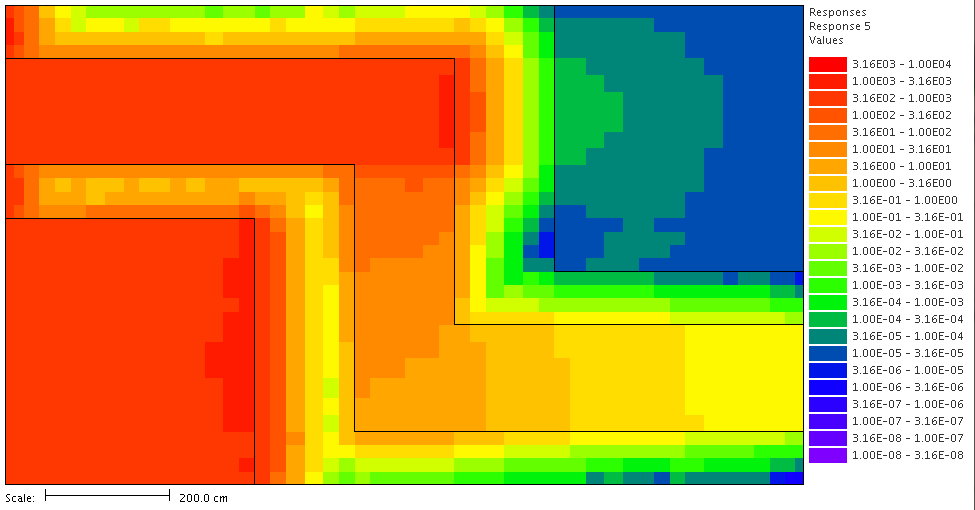
\includegraphics[height=1.1in,clip]{../figs/labyrinth-dr}
		%\caption{}
	\end{center}
  	\end{figure}
  \end{column}
\end{columns}

\end{frame}


% --------------------------------------------------------------
% --------------------------------------------------------------
\section{\scshape Motivation}
%\subsection{Motivation}
\begin{frame}[fragile]
  \frametitle{Project motivation}

\begin{columns}
  \begin{column}{0.55\textwidth}
	\begin{itemize}
	\item Need to accurately model radiation for safeguarding and monitoring
	\item \alert{Challenging}: dense shields; streaming paths
	\item Current methods are insufficient
	\item \alert{Goal}: accurate solutions in reasonable time
	\item New methods can easily be added to existing codes
	\end{itemize}
  \end{column}
  \begin{column}{0.45\textwidth}
  	\begin{figure}
  	\begin{center}
  		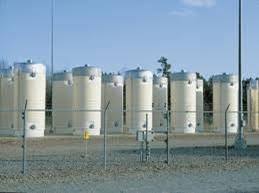
\includegraphics[height=1.25in,clip]{../figs/isfsi}
		%\caption{}
	\end{center}
  	\end{figure}
  \end{column}
\end{columns}

\end{frame}

% --------------------------------------------------------------
% --------------------------------------------------------------
\begin{frame}[fragile]
  \frametitle{Solving the TE}
%
\begin{columns}
  \begin{column}{0.5\textwidth}
  \begin{center}
  \underline{Monte Carlo}
  \end{center}
	\begin{itemize}
	\item Solution has statistical error
	\item \textit{Continuous} phase space: ``gold standard answers"
	\item Can be slow
	\item Optically thick = \textit{slow}
	\end{itemize}
  \end{column}
  \begin{column}{0.5\textwidth}
  \begin{center}
  \underline{Deterministic}
  \end{center}
	\begin{itemize}
	\item Solution equally valid everywhere
	\item \textit{Discretized} phase space: drives solution quality
	\item Can be fast
	\item Streaming = \textit{ray effects}
	\end{itemize}
  \end{column}
\end{columns}
%
\begin{align}
\vOmega \cdot \nabla \psi(\vec{r}, E, \vOmega) &+
\Sigma_t \psi(\vec{r}, E, \vOmega) = S(\vec{r}, E, \vOmega) \:+\nonumber\\
%
& \int_{4\pi} d\vOmega' \int_0^{\infty} dE'\: \Sigma_s(E', \vOmega' \rightarrow E, \vOmega) \psi(\vec{r}, E', \vOmega') \nonumber
\end{align}

\end{frame}

% --------------------------------------------------------------
\begin{frame}[fragile]
  \frametitle{Acceleration}
  \begin{itemize}
  	\item To use MC in many applications, we need to \textit{accelerate} it
	\item Variance reduction is designed to improve the FOM:
  \end{itemize}
\begin{align}
\text{FOM} = \frac{1}{\text{R}^2\text{t}} \qquad & \text{R = relative error} \nonumber \\ 
& \text{t = time} \nonumber 
\end{align}
  \begin{itemize}
  	\item \underline{Idea}: can we use deterministic and Monte Carlo methods together to lessen the weaknesses of each?
  \end{itemize}
  \pause
  $\rightarrow$ \textbf{Hybrid Methods}

\end{frame}


% --------------------------------------------------------------
\section{\scshape Hybrid Methods}
%\subsection{CADIS}
\begin{frame}[fragile]
  \frametitle{Forward-adjoint relationship}
Define response with function $f(\ve{r}, E)$ in volume $V_r$ as
%
\begin{equation}
 R = \int_E \int_{V_r} f(\ve{r}, E) \phi(\ve{r}, E)\: dV dE 
 \label{eq:Response}
\end{equation}
%
\begin{columns}
  \begin{column}{0.45\textwidth}
	\begin{align}
  	H\phi &= q \quad \text{(forward)}\nonumber \\
  	%
  	H^{\dagger} \phi^{\dagger} &= q^{\dagger} \quad 
  	\text{(adjoint)}\nonumber
  	\end{align}
  \end{column}
  \begin{column}{0.45\textwidth}
  	\begin{align}
  	\langle H\phi, \phi^{\dagger} \rangle &= \langle H^{\dagger} \phi^{\dagger}, \phi \rangle \:, \text{and therefore} \nonumber \\
  	%
  	\langle q, \phi^{\dagger} \rangle &= \langle q^{\dagger}, \phi \rangle \nonumber
  	\end{align}
  \end{column}
\end{columns}
\vspace*{1 em}
\pause
If we let $q^{\dagger} = f(\ve{r}, E)$, then
%
\begin{equation}
 \langle q^{\dagger}, \phi \rangle = \langle f, \phi \rangle = R = \langle q, \phi^{\dagger} \rangle 
 \label{eq:ResponseRedef}
\end{equation}
%
Eq.\ \eqref{eq:ResponseRedef} expresses that $\phi^{\dagger}$ represents the expected contribution of a source particle to the response given the source, $q$.

\end{frame}

% --------------------------------------------------------------
\begin{frame}[fragile]
  \frametitle{CADIS \cite{Wagner2007}}
  
  \begin{enumerate}
  \item Define $q^{\dagger}$ as the local response of interest\\
  \item Coarse deterministic calculation to get $\phi^{\dagger}$ and $R$
  \end{enumerate}
% 
\begin{align*}
  imp(\ve{r}, E) &= \frac{\phi^{\dagger}(\ve{r}, E)}{\langle q(\ve{r}, E), \phi^{\dagger}(\ve{r}, E) \rangle} = \frac{\phi^{\dagger}(\ve{r}, E)}{R} \\
  %
  \hat{q}(\ve{r}, E) &= \frac{\phi^{\dagger}(\ve{r}, E) q(\ve{r}, E)}{R} \\
  %
  w_0(\ve{r}, E) &= \frac{q(\ve{r}, E)}{\hat{q}(\ve{r}, E)} = \frac{R}{\phi^{\dagger}(\ve{r}, E)} 
  \label{eq:Importance}
\end{align*}

Birth weights match weight targets: \underline{C}onsistent \underline{A}djoint \underline{D}riven \underline{I}mportance \underline{S}ampling \underline{M}ethod

\end{frame}

% --------------------------------------------------------------
%\subsection{FW-CADIS}
\begin{frame}[fragile]
  \frametitle{FW-CADIS \cite{Wagner2007}}

\begin{itemize}
\item We often what to optimize solutions in all of phase space\\
\item In this case the adjoint source needs to be a global forward solution: \underline{F}orward \underline{W}eighted-CADIS
\end{itemize}
%
\begin{columns}
  \begin{column}{0.5\textwidth}
  \begin{center}
  \textcolor{byellow}{To Optimize}
  \end{center}
	\begin{align}
  	&\phi(\ve{r}, E)\nonumber \\
  	%
  	\int&\phi(\ve{r}, E)\sigma_d(\ve{r}, E)\nonumber
  	\end{align}
  \end{column}
  %
  \begin{column}{0.5\textwidth}
  \begin{center}
  \textcolor{byellow}{Adjoint Source}
  \end{center}
  	\begin{align}
  	f(\ve{r}, E) &= \frac{1}{\phi(\ve{r}, E)}\nonumber \\
  	%
  	f(\ve{r}, E) &= \frac{\sigma_d(\ve{r}, E)}{\int\phi(\ve{r}, E)\sigma_d(\ve{r}, E)} \nonumber
  	\end{align}
  \end{column}
\end{columns}
\vspace*{1 em}
\pause
For example
%
\begin{equation}
 R = \int_E \int_{V_f} f(\ve{r}, E) \phi(\ve{r}, E) dV dE = \int_E \int_{V} \frac{1}{\phi(\ve{r}, E)} \phi(\ve{r}, E) dV dE \approx 1 \nonumber
\end{equation}

\end{frame}

% --------------------------------------------------------------
%\subsection{Challenges}
\begin{frame}[fragile]
  \frametitle{Challenges}

	FW-CADIS works well for \textbf{most} shielding problems...
	%
	\begin{columns}
  	\begin{column}{0.5\textwidth}
  	\begin{figure}
  	\begin{center}
  		\includegraphics[height=2in,clip]{../figs/dlvn}
		\caption{Dog Legged Void Neutron shielding benchmark}
	\end{center}
  	\end{figure}
  	\end{column}
 	%
 	\begin{column}{0.5\textwidth}
 	\begin{figure}
  	\begin{center}
  		\includegraphics[height=2in,clip]{../figs/dlvn-lowVR}
  		\caption{MC 95\% CI RE using FW-CADIS, DLVN \cite{Slaybaugh2013}}
  	\end{center}
  	\end{figure}
  	\end{column}
	\end{columns}
  
\end{frame}

% --------------------------------------------------------------
\begin{frame}[fragile]
  \frametitle{Challenges}

	...but not \textbf{all} of them
	%
	\begin{columns}
  	\begin{column}{0.45\textwidth}
  	\begin{center}
  	\begin{figure}
  		\includegraphics[height=2in,clip]{../figs/plate-badVR}
  		\caption{MC 95\% CI RE using FW-CADIS, plate \cite{Wilson2015}}
  	\end{figure}
	\end{center}
  	\end{column}
 	%
 	\begin{column}{0.5\textwidth}
  	\begin{center}
  	\begin{itemize}
		\item FW-CADIS only includes space and energy, \textit{not angle}
		\pause
		\item An example case: fission spectrum source with long streaming path
		\item High relative error through location of interest
		\pause
		\item Capturing angular behavior will help improve the solution
	\end{itemize}
  	\end{center}
  	\end{column}
	\end{columns}
  
\end{frame}


% --------------------------------------------------------------
% --------------------------------------------------------------
\begin{frame}[fragile]
  \frametitle{Anisotropy: a computational challenge}

	\begin{columns}
  	\begin{column}{0.5\textwidth}
	\begin{itemize}
	\item Many important nuclear applications have strong anisotropies
	 \begin{itemize}
	 \item \textbf{Used fuel casks}
	 \item Reprocessing facilities
	 \item Reactor facilities
	 \item Active interrogation 
	 \end{itemize}
	\pause
	\item These are difficult to capture with current tools:
	 \begin{itemize}
	 \item Ray effects with deterministic
	 \item Too slow with analog MC
	 \item Insufficient acceleration of MC with hybrid
	 \end{itemize}
	\end{itemize}
  	\end{column}
 	%
 	\begin{column}{0.5\textwidth}
 	 \begin{center}
 	 \begin{figure}
 	 \includegraphics[height=2in,clip]{../figs/pwr}  
 	 \caption{PWR relative error \cite{Pantelias2013}}
 	 \end{figure}
 	 \end{center}

  	\end{column}
	\end{columns}

\end{frame}


% --------------------------------------------------------------
\section{Strong Anisotropies}
\begin{frame}[fragile]
  \frametitle{Current hybrid methods are insufficient}

	\begin{itemize}
	\item MC VR parameters created from adjoint deterministic scalar flux that is a function of \textit{space and energy only} \vspace*{1 em}
	\item Angular dependence of the importance function is not retained, otherwise the map would be 
	\begin{itemize}
	  \item very large (tens or hundreds of GB) and
	  \item  more costly and complex to use in the Monte Carlo simulation 
	\end{itemize}
	\item Drawback: within a given space/energy cell, the map provides the average importance of a particle moving in \textit{any direction} through the cell -- excluding information about how particles move \alert{toward the objective}
	\end{itemize}

\end{frame}

% --------------------------------------------------------------
\begin{frame}[fragile]
  \frametitle{Current hybrid methods are insufficient}

	\begin{columns}
  	\begin{column}{0.5\textwidth}
 	 \begin{center}
 	 \begin{figure}
 	 \includegraphics[height=2in,clip]{../figs/boat-interrogation}  
 	 \caption{Spherical boat model with source on left and fissionable material at center}
 	 \end{figure}
 	 \end{center}
  	\end{column}
 	%
 	\begin{column}{0.5\textwidth}
 	 \begin{center}
 	 \begin{figure}
 	 \includegraphics[height=2in,clip]{../figs/boat-map}  
 	 \caption{Target weight window values for 14.1 MeV neutrons}
 	 \end{figure}
 	 \end{center}
  	\end{column}
	\end{columns}

\end{frame}

% --------------------------------------------------------------
\begin{frame}[fragile]
  \frametitle{Many attempts at resolution $\rightarrow$ \\ 
  \hspace*{3em} Limited Success}

	\begin{itemize}
	\item Automatic WW generator in MCNP \cite{MCNP2008}
	\item AVATAR \cite{vanRiper1997}
	\item LIFT \cite{Turner1997}
	\item Cooper and Larsen's global weight windows \cite{Cooper2001}
	\item FW/CADIS
	\item Resonance Factor method \cite{Wilson2015}
	\end{itemize}
	
\vspace*{1 em}
\textit{Better hybrid methods are needed}; \alert{two ideas}.

\end{frame}

% --------------------------------------------------------------
\begin{frame}[fragile]
  \frametitle{Integration weighting}

    Different integration plan captures angles in scalar flux creation	
	\begin{align*}
		\phi^{\dagger}(\ve{r},E) &= \int \psi^{\dagger}(\vOmega, 
		\ve{r},E) d\vOmega \qquad  \qquad \qquad \text{original}\\
		 %
		\phi^{\dagger}(\ve{r},E) &= \frac{\int \psi(\vOmega, \ve{r},E)
		 \psi^{\dagger}(\vOmega, \ve{r},E) d\vOmega}{\int \psi(\vOmega, 
		 \ve{r},E)  d\vOmega} \qquad \text{new}
	\end{align*}

    \pause
    Major challenges and areas of investigation:
	\begin{enumerate}
	\item Data storage and handling (many GBs)
	\item More, less, or differently sensitive to 
	  \begin{itemize}
	  \item quality of the discrete ordinates calculation?
	  \item ray effects?
	  \end{itemize}
	\end{enumerate}

\end{frame}

% --------------------------------------------------------------
\begin{frame}[fragile]
  \frametitle{Lagrange discrete ordinate equations}

    Use a formulation that is more flexible in the ways that 
	it handles quadrature: new LDO equations \cite{Ahrens2014}
	\vspace*{1 em}
	
	\begin{itemize}
	\item Re-derivation of $S_N$ with an \alert{interpolatory quadrature framework}
	\item Allows evaluation at directions not on quadrature set
	\item Can use \alert{asymmetric angles}
	\item No need to store spherical harmonic moments
	\item May be useful for more accurately capturing strong anisotropies
	\end{itemize}

\end{frame}

% --------------------------------------------------------------
\begin{frame}[fragile]
  \frametitle{Method implementation}

  	\begin{itemize}
    \item The space- and energy-dependent importance map will be normalized and 
     source biasing parameters will be generated in the \alert{same ways} as
     the current implementation of FW/CADIS \vspace*{1 em}
	\item Immediately useful; widely applicable \vspace*{1 em}
	\item We will study both strategies and characterize the impact\vspace*{1 em}
	\item Will be available in SCALE \cite{SCALE} and ADVANTG \cite{Pantelias2013}
	\end{itemize}
	
\end{frame}

% --------------------------------------------------------------
\begin{frame}[fragile]
  \frametitle{Application problems}


	
\end{frame}


% --------------------------------------------------------------
% --------------------------------------------------------------
\section{Status and Plan}
\begin{frame}[fragile]
  \frametitle{Status and plan}


	
\end{frame}


% --------------------------------------------------------------
% --------------------------------------------------------------
\section*{}
\begin{frame}[fragile]
  \frametitle{Questions?}
  \begin{center}
  \includegraphics[height=3in,clip]{../questions-comic}  
  \end{center}
  
\end{frame}

% --------------------------------------------------------------
\begin{frame}[allowframebreaks]{References}
	\bibliographystyle{unsrt}
	\bibliography{2015-03-mpact}
\end{frame}

\end{document}
